\documentclass{beamer}
\mode<presentation>
{
  \usepackage{theme/theme}
  \setbeamercovered{transparent}
}

\usepackage{amsmath,amssymb,amsfonts}
\usepackage{times}
\usepackage{graphicx}
\usepackage{fancyvrb}
\usepackage{array}
\usepackage{colortbl}
\usepackage{tabularx}
\usepackage{fontspec}
\usepackage{minted}

% Uncomment me when you need to insert code
\usepackage{color}
\usepackage{listings}
% End Code

% End Header

% Titlepage
\newcommand{\maintitle}{T7. Distributed Systems}
\title{\maintitle}
\author{Enterprise Software Architectures}
\institute
{
  Bachelor's Degree in Computer Engineering
}
\date{Academic year 2025/26}
% End Titlepage

\AtBeginSection[]{
  \begin{frame}
    \centering
    \begin{beamercolorbox}[sep=8pt,center]{title}
      \usebeamerfont{title}\insertsectionhead
    \end{beamercolorbox}
  \end{frame}
}

% Slides
\begin{document}

\begin{frame}
  \titlepage
\end{frame}

\begin{frame}
  \frametitle{\maintitle}
  \tableofcontents[subsectionstyle=show]
\end{frame}

\section{Block A - Scalability}

\begin{frame}
  \frametitle{The need for scalability}

  "A while back, you built a simple application and deployed it on a single server. It worked great for the first few users, but as word spread and traffic increased, you started noticing problems..."
  \newline

  \begin{itemize}
    \item CPU and memory usage increase.
    \item Response times grow and requests start timing out.
    \item The server eventually crashes under peak load.
  \end{itemize}
\end{frame}

\begin{frame}
  \frametitle{The need for scalability}

  We need a strategy to handle \textbf{ever increasing load} without degrading the user experience.

  \begin{itemize}
    \item \textbf{Application-level optimizations}
    \begin{itemize}
      \item Find and optimize bottlenecks in the code.
      \item \textbf{Problem:} This can only get you so far. Eventually, you will hit the limits of what a single server can handle.
    \end{itemize}
    \item \textbf{Scale the architecture}
    \begin{itemize}
      \item Increase capacity by adding more servers and distributing the load across them.
    \end{itemize}
  \end{itemize}

  \begin{exampleblock}{Note}
    Scalable architectures introduce significant complexity and cost. Some applications (like \textit{internal tools}) don't need to be scalable.
  \end{exampleblock}
\end{frame}

\subsection{Application Scaling and Load Balancing}

\begin{frame}
  \frametitle{Vertical vs. Horizontal Scaling}

  \textbf{Vertical scaling} (scale up): replace the server with a bigger one.
  \begin{columns}
    \column{0.6\textwidth}
    \begin{itemize}
      \item \textbf{Fast and simple}: no code changes required.
      \item Has a \textbf{hard ceiling}: you can only buy so much hardware.
      \item Creates a \textbf{single point of failure}.
    \end{itemize}

    \column{0.4\textwidth}
    \centering
    \begin{figure}
      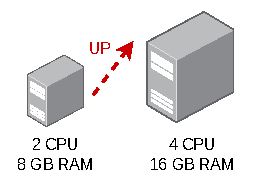
\includegraphics[width=\textwidth]{images/T7/vertical-scaling.pdf}
      \caption{Vertical scaling}
    \end{figure}
  \end{columns}

\end{frame}

\begin{frame}
  \frametitle{Vertical vs. Horizontal Scaling}

  \textbf{Horizontal scaling} (scale out): add more instances of the service.
  \begin{columns}
    \column{0.6\textwidth}
    \begin{itemize}
      \item Virtually \textbf{unlimited} capacity.
      \item Built-in \textbf{redundancy}: one failing instance does not take the whole system down.
      \item Usually requires a \textbf{load balancer} to distribute traffic evenly.
      \item Can add/remove instances dynamically (\textbf{auto-scaling}).
    \end{itemize}

    \column{0.4\textwidth}
    \centering
    \begin{figure}
      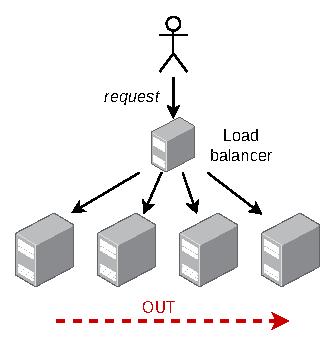
\includegraphics[width=\textwidth]{images/T7/horizontal-scaling.pdf}
      \caption{Horizontal scaling}
    \end{figure}
  \end{columns}

\end{frame}

\begin{frame}
  \frametitle{Load Balancing Strategies}

  A \textbf{load balancer} sits in front of the server instances\footnote{Other load balancing solutions exist, such as DNS-based load balancing or floating IPs.} and distributes incoming requests according to a routing algorithm.
  \newline

  Some common strategies:

  \begin{itemize}
    \item \textbf{Round-robin}: requests are distributed in order, one per instance.
    \item \textbf{Least connections}: the instance with the fewest active requests is chosen.
    \item \textbf{IP hash}: the client's IP address determines which instance handles the request
      (useful for \textit{sticky sessions}).
  \end{itemize}

\end{frame}

\begin{frame}
  \frametitle{Auto-scaling}

  Instead of manually adding instances, \textbf{auto-scaling} policies react to metrics
  in real time:

  \begin{itemize}
    \item \textbf{CPU-based}: average/P95 CPU usage of all instances.
    \item \textbf{Request-rate-based}: number of requests per second per instance.
    \item \textbf{Response-time-based}: average/median/P95 latency.
  \end{itemize}

  \begin{block}{Containerization}
    Using Docker or similar technologies greatly simplifies auto-scaling, as containers can be started and stopped easily.
  \end{block}

\end{frame}

\subsection{Database Scaling}

\begin{frame}
  \frametitle{Database Scaling}

  Scaling application servers is (relatively) straightforward. However, a database cannot be scaled the same way because it holds \textbf{shared mutable state}.
  \newline

  Two main strategies to scale databases:
  \begin{itemize}
    \item \textbf{Replication}: create read-only copies of the database to distribute read load.
    \item \textbf{Sharding}: partition the database into smaller pieces (shards) that can be distributed across multiple servers.
  \end{itemize}

\end{frame}

\begin{frame}
  \frametitle{Database Replication}

  Database load is often read-heavy: many more read queries than write queries.
  Replication creates one or more read-only copies (\textit{replicas}) of the \textbf{full database}.
  
  \begin{columns}
    \column{0.45\textwidth}
    \begin{itemize}
      \item The \textbf{primary} handles all \textit{write} operations.
      \item \textbf{Replicas} serve \textit{read} operations, distributing the read load.
    \end{itemize}

    \column{0.5\textwidth}
    \centering
    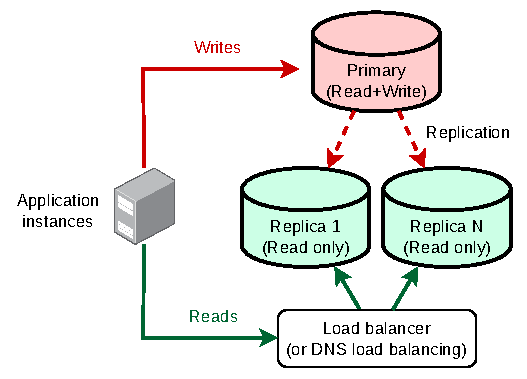
\includegraphics[width=\textwidth]{images/T7/db-replication.pdf}
  \end{columns}

\end{frame}

\begin{frame}
  \frametitle{Replication Lag and Eventual Consistency}

  Replication is not instantaneous. There is always a small \textbf{replication lag} between a write on the primary and its appearance on the replicas.

  \begin{itemize}
    \item Writing a value and then immediately reading it may return the old value (\textit{stale read}).
  \end{itemize}

  \begin{block}{Eventual Consistency}
    The system guarantees that, \textit{given enough time without new writes}, all replicas
    will converge to the same value. Data is \textbf{not immediately consistent}, but it will
    \textbf{eventually} be.
  \end{block}

\end{frame}

\begin{frame}
  \frametitle{The CAP Theorem}

  It has been proven that a distributed system (usually a DB cluster) can guarantee \textbf{at most two} of the following three properties:

  \begin{itemize}
    \item \textbf{Consistency (C)}: Every read receives either the most recent write or an error (never stale data).
    \item \textbf{Availability (A)}: Every request to a working node receives a non-error response (even if the data is stale).
    \item \textbf{Partition tolerance (P)}: The system continues to operate despite network partitions\footnote{A network partition is any situation where some nodes cannot communicate with others (e.g., due to a network failure).}.
  \end{itemize}

\end{frame}

\begin{frame}
  \frametitle{The CAP Theorem}

  Network partitions are \textit{unavoidable} in real life. The real trade-off is between \textbf{Consistency} and \textbf{Availability} during a partition.
  \newline

  When a connectivity issue is detected in the cluster, you must choose to either:
  \begin{itemize}
    \item Prioritize \textbf{Availability}: continue serving requests, returning stale data (AP system).
    \begin{itemize}
      \item \textit{Examples:} Apache Cassandra, CouchDB, AWS DynamoDB
    \end{itemize}
    \item Prioritize \textbf{Consistency}: reject requests (CP system).
    \begin{itemize}
      \item \textit{Examples:} MongoDB, Redis, Apache HBase
    \end{itemize}
  \end{itemize}

\end{frame}

\begin{frame}
  \frametitle{Database Sharding}

  \textbf{Replication} solves the \textit{read} bottleneck, but all writes still go to one node. \textbf{Sharding} solves the \textit{write} bottleneck by \textbf{horizontally partitioning} data across multiple database instances (\textit{shards}).

  \begin{columns}
    \column{0.5\textwidth}
    
    Each shard holds a \textbf{subset of the rows}, determined by a \textit{shard key} (e.g., user ID range, geographic region, hash of the key).

    \column{0.5\textwidth}
    \centering
    \begin{figure}
      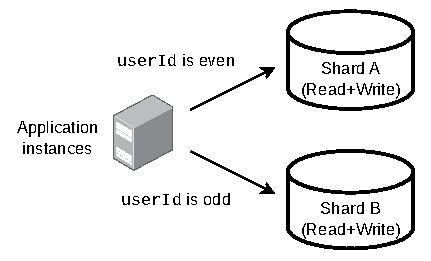
\includegraphics[width=\textwidth]{images/T7/db-sharding.pdf}
      \caption{Sharding by user ID.}
    \end{figure}
  \end{columns}

\end{frame}

\begin{frame}
  \frametitle{Database Sharding}

  \textbf{Disadvantages:}
  \begin{itemize}
    \item Queries that span multiple shards require \textbf{aggregation} at the application level. This is very complex and slow.
    \item Choosing a good shard key is hard. A poor choice leads to extremely \textbf{low performance}.
    \item Changing the partition scheme (known as \textbf{resharding}) is slow and complex.
  \end{itemize}

\end{frame}

\begin{frame}
  \frametitle{Which one should I use?}

  \begin{columns}
    \column{0.33\textwidth}
    \centering
    \textbf{Low overall load}
    \begin{figure}
      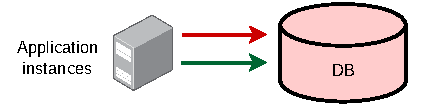
\includegraphics[width=0.8\textwidth]{images/T7/db-single-node.pdf}
    \end{figure}
    Single node (use Vertical scaling)
    \column{0.33\textwidth}
    \centering
    \textbf{Read-heavy load}
    \begin{figure}
      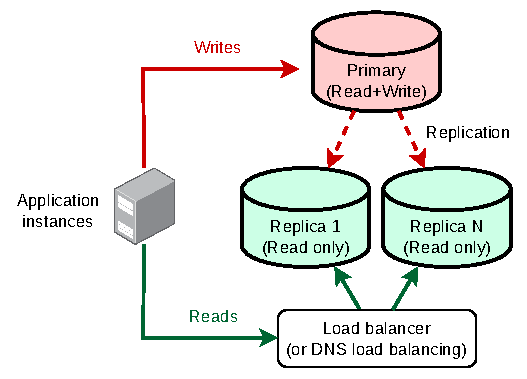
\includegraphics[width=1\textwidth]{images/T7/db-replication.pdf}
    \end{figure}
    Just Replication
    \column{0.33\textwidth}
    \centering
    \textbf{Very high read+write load}
    \begin{figure}
      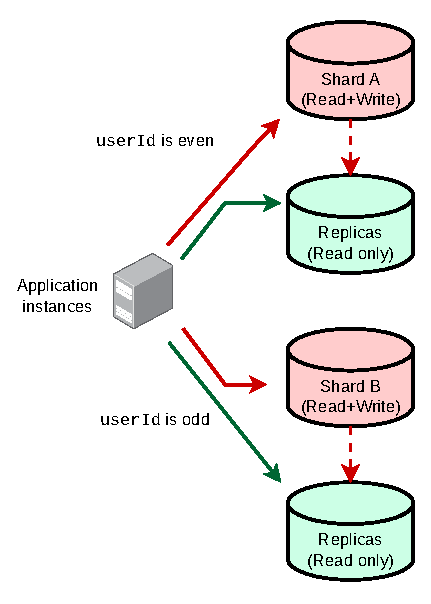
\includegraphics[width=0.75\textwidth]{images/T7/db-sharding-replication.pdf}
    \end{figure}
    Sharding (scalability) + Replication (resilience)
  \end{columns}

\end{frame}

\subsection{Caching}

\begin{frame}
  \frametitle{Caching}

  A \textbf{cache} stores the results of expensive operations so that subsequent requests can be served faster without hitting the database.
  \newline

  Two levels of caching are commonly used together:

  \begin{itemize}
    \item \textbf{L1 (In-process cache)}: stored in the application's RAM.
    \begin{itemize}
      \item Fastest possible access, but \textbf{not shared} between instances.
      \item Lost when the process restarts.
      \item Examples: a simple \texttt{HashMap}, Caffeine, Guava Cache.
    \end{itemize}
    \item \textbf{L2 (Distributed cache)}: a shared external cache.
    \begin{itemize}
      \item Shared across all instances.
      \item Slower than L1 (requires a network call), but much faster than a DB query.
      \item Examples: Redis, Memcached.
    \end{itemize}
  \end{itemize}

\end{frame}

\begin{frame}
  \frametitle{Caching Architecture Example}

  \centering
  \begin{figure}
    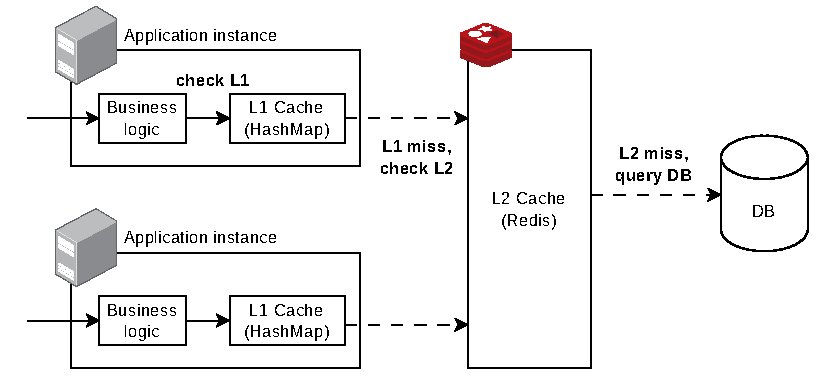
\includegraphics[width=\textwidth]{images/T7/cache-layers.pdf}
    \caption{A DB cache architecture using HashMap for L1 and Redis for L2.}
  \end{figure}

\end{frame}

\begin{frame}
  \frametitle{Cache Invalidation Strategies}

  Getting cached data \textbf{out-of-date} is the main risk of caching. Common invalidation strategies:

  \begin{itemize}
    \item \textbf{TTL (Time-To-Live)}: cached entries expire automatically after a fixed duration.
    \begin{itemize}
      \item Simple, but \textbf{TTL is arbitrary} and may serve stale data.
    \end{itemize}
    \item \textbf{Write-through}: the cache is updated synchronously on every write to the DB.
    \begin{itemize}
      \item Cache is always fresh, but write latency increases.
    \end{itemize}
    \item \textbf{Write-behind (write-back)}: writes go to the cache first, the DB is updated asynchronously.
    \begin{itemize}
      \item Fast writes, but risk of data loss on cache failure.
    \end{itemize}
  \end{itemize}

\end{frame}

\subsection{Content Delivery Networks}

\begin{frame}
  \frametitle{Content Delivery Networks (CDNs)}

  Some data \textbf{doesn't change frequently} and is expensive to retrieve or generate.
  \newline

  \begin{block}{Examples}
    \begin{itemize}
      \item \textbf{Static assets} like images, videos, CSS, JS, static HTML...
      \item Results of \textbf{expensive computations} that are worth caching for a long time: \texttt{GET} API responses, rendered HTML...
    \end{itemize}

  \end{block}

\end{frame}

\begin{frame}
  \frametitle{Content Delivery Networks (CDNs)}

  \begin{figure}
    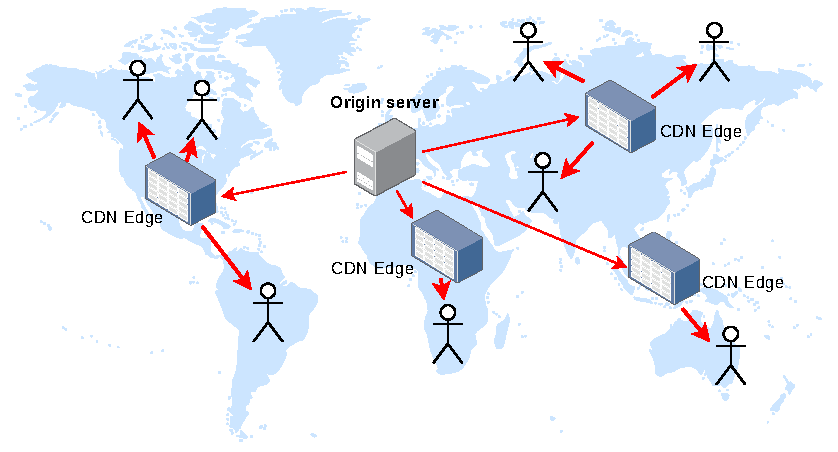
\includegraphics[height=0.5\textheight]{images/T7/cdn.pdf}
  \end{figure}

  \begin{itemize}
    \item Reduces \textbf{latency} by serving from the nearest edge location.
    \item Greatly reduces \textbf{load} on the origin servers.
    \item Can provide \textbf{DDoS protection} and \textbf{WAF} features.
  \end{itemize}

\end{frame}

\section{Block B - Distribution and Communication Strategies}

\subsection{Monolith vs. Microservices}

\begin{frame}
  \frametitle{Monolith}

  A monolith packages all application functionality into a \textbf{single deployable unit}\footnote{A monolith is \textbf{not} necessarily \textit{tightly coupled}, it can be modularized and have clear interfaces, but they are \textit{logical} boundaries, not \textit{physical} ones.} in order to \textbf{minimize remote calls}. In-process function calls are orders of magnitude faster than network calls.
  \newline

  \begin{figure}
    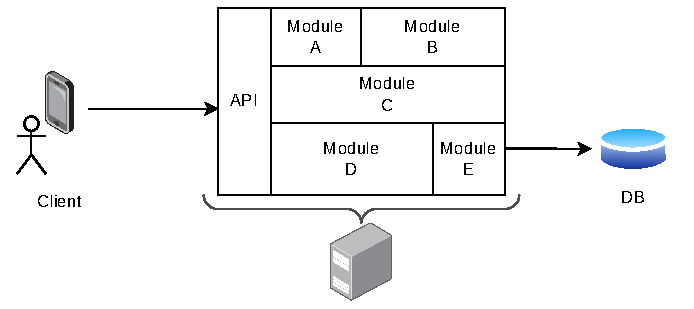
\includegraphics[height=0.45\textheight]{images/T7/monolith.pdf}
  \end{figure}
  
\end{frame}

\begin{frame}
  \frametitle{Microservices}

  Microservices decompose the system into small, \textbf{independently deployable} services, each with its \textbf{own database}.
  \newline

  \begin{figure}
    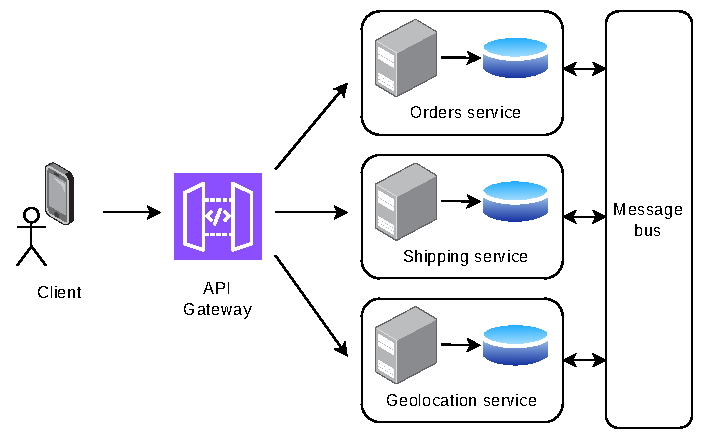
\includegraphics[height=0.6\textheight]{images/T7/microservices.pdf}
  \end{figure}

\end{frame}

\begin{frame}
  \frametitle{Microservices}

  \textbf{Advantages:}
  \begin{itemize}
    \item Each service can be \textbf{deployed and scaled independently}.
    \item Services can be developed by different teams and using different technologies.
  \end{itemize}

  \textbf{Disadvantages:}
  \begin{itemize}
    \item Increased operational \textbf{complexity and cost}.
    \item Network calls are slow and can fail.
    \item Maintaining data consistency across multiple DBs is hard.
    \item Debugging a request that spans 10 services is much harder than debugging a monolith.
  \end{itemize}

\end{frame}

\begin{frame}
  \frametitle{Serverless Functions}

  Serverless architectures or \textit{Functions as a Service (FaaS)} take this idea further: each \textbf{function} is deployed and scaled independently, with \textbf{no infrastructure management}.

  \begin{itemize}
    \item The cloud provider handles scaling.
    \item You pay only for actual execution time.
  \end{itemize}

  \textbf{Disadvantages:}
  \begin{itemize}
    \item \textbf{Cold start latency}: the first request after a period of inactivity is slow while the runtime initializes.
    \item Best suited for \textbf{short-lived, event-driven tasks}, not for complex or long processes.
    \item Vendor lock-in.
  \end{itemize}

\end{frame}

\begin{frame}
  \frametitle{Which architecture to use?}

  \begin{block}{Recommendation}
    \textbf{Start with a monolith}. Extract services progressively, only when a clear need arises (e.g., a specific module needs independent scaling or a dedicated team).
  \end{block}

  \textbf{Why?}
  \begin{itemize}
    \item In the early stages of a project, requirements change rapidly. A monolith is much easier to refactor.
    \item Microservices are harder to build correctly, and their benefits only materialize at a certain scale.
    \item A well-modularized monolith can be broken apart later.
  \end{itemize}

\end{frame}

\subsection{Communication Patterns}

\begin{frame}
  \frametitle{Synchronous vs asynchronous communication}

  \textbf{Synchronous}: the caller \textbf{waits} for the response before continuing.

  \begin{itemize}
    \item Simple and intuitive, suitable for request-response interactions.
    \item \textbf{Trade-off}: If the called service is slow or unavailable, the caller is blocked. Can lead to cascading failures if not handled properly.
  \end{itemize}
  {\color{white} . }

  \textbf{Asynchronous}: the caller sends a message and continues without waiting for a response. A \textbf{message broker} mediates the communication.
  \begin{itemize}
    \item When all services \textit{react to events} rather than making synchronous calls, we have an \textbf{event-driven architecture}.
  \end{itemize}

\end{frame}


\begin{frame}
  \frametitle{Asynchronous communication patterns}

  \textbf{Message Queue}: messages are placed in a queue and consumed by \textit{one} service (N $\rightarrow$ 1).
  \begin{itemize}
    \item Messages persist until the consumer has fully processed them.
    \begin{itemize}
      \item Very resilient to consumer failures.
      \item Higher latency (\texttt{C} must wait until \texttt{A} and \texttt{B} have finished).
    \end{itemize}
    \item Examples: RabbitMQ, AWS SQS.
  \end{itemize}
  {\color{white} . }

  \begin{figure}
    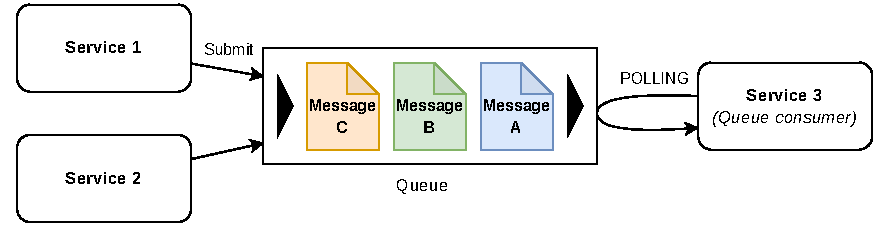
\includegraphics[width=0.85\textwidth]{images/T7/message-queue.pdf}
  \end{figure}

\end{frame}

\begin{frame}
  \frametitle{Asynchronous communication patterns}

  \textbf{Publish/Subscribe (Pub/Sub)}: services publish \textit{real-time events} to a \textit{topic}, all subscribed services receive a copy (N $\rightarrow$ N).
  \begin{itemize}
    \item Messages are \textit{transient}: if a subscriber is down, it will miss messages published during that time.
    \item Examples: Apache Kafka, AWS SNS, Google Pub/Sub.
  \end{itemize}

  \begin{figure}
    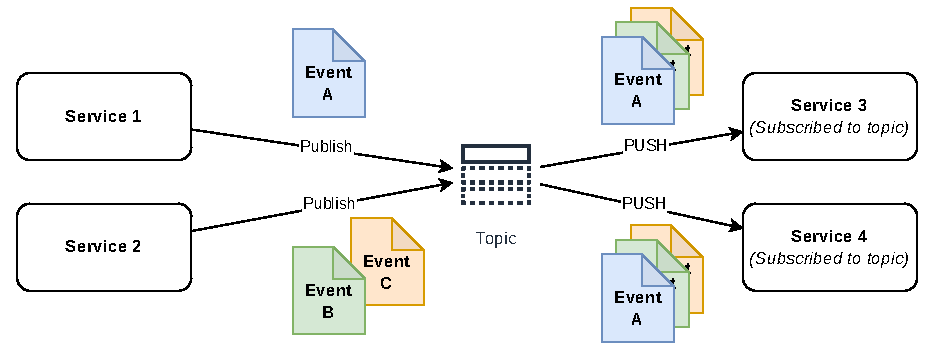
\includegraphics[width=0.8\textwidth]{images/T7/pub-sub.pdf}
  \end{figure}

\end{frame}

\begin{frame}
  \frametitle{Asynchronous communication patterns}

  \textbf{Advantages:}
  \begin{itemize}
    \item \textbf{Decoupling} between publishers and subscribers.
    \begin{itemize}
      \item They don't need to know about each other.
      \item In a message queue, they don't even need to be available at the same time.
    \end{itemize} 
    \item \textbf{Resilience}: messages are buffered in the broker.
    \begin{itemize}
      \item A subscriber can be down temporarily without losing messages.
      \item A sudden spike in traffic can be absorbed by the queue.
    \end{itemize}
  \end{itemize}

  \textbf{Disadvantages:}
  \begin{itemize}
    \item Higher \textbf{latency}, especially with message queues.
    \item Complex \textbf{debugging}: requests don't follow a linear call path.
    \item Requires additional \textbf{infrastructure} (message broker).
  \end{itemize}

\end{frame}

\subsection{Failure Handling}

\begin{frame}
  \frametitle{Failure is inevitable}

  In a distributed system, \textbf{partial failures} are the norm.

  A well-designed system should be able to \textbf{gracefully degrade}\footnote{\textit{Graceful degradation}: only the functionality that depends on the failing service is affected, while the rest of the system continues to operate normally.} when one or more services are slow or unavailable.
  \newline

  Several patterns help us build \textbf{resilient} systems:
  \begin{enumerate}
    \item Circuit Breaker
    \item Timeouts + retries with exponential backoff
    \item Rate limiting and backpressure
    \item Idempotency
  \end{enumerate}

\end{frame}

\begin{frame}
  \frametitle{Circuit Breaker pattern}

  A \textbf{proxy} sits between the caller and the callee, and \textbf{trips open}\footnote{Electrical circuit breakers \textit{open} the circuit when a fault is detected.} (stops requests) when too many failures are detected.

  \begin{itemize}
    \item Prevents the caller from waiting in useless requests.
    \item Gives the failing service room to automatically recover, by reducing its load until it is healthy again.
  \end{itemize}

  \begin{figure}
    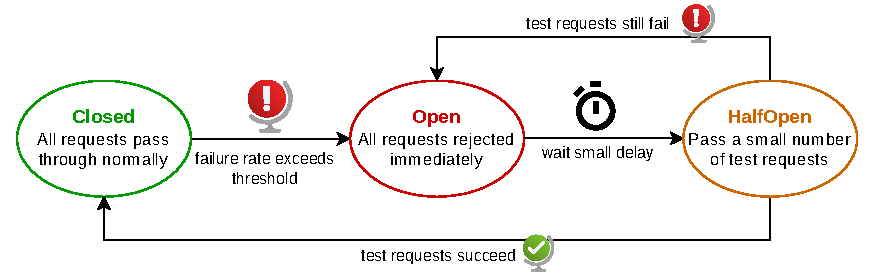
\includegraphics[width=0.9\textwidth]{images/T7/circuit-breaker.pdf}
  \end{figure}

\end{frame}

\begin{frame}
  \frametitle{Circuit Breaker states}

  \begin{itemize}
    \item \textbf{Closed} (normal): requests pass through. Failures are counted. When the failure rate exceeds a threshold, the circuit \textit{trips open}.
    \item \textbf{Open} (fast-fail): all requests are \textbf{rejected immediately} without calling the downstream service. After a timeout, the circuit moves to \textit{half-open}.
    \item \textbf{Half-Open} (testing): a \textbf{limited number of test requests} are allowed through.
      \begin{itemize}
        \item If they succeed: the circuit \textit{closes} (service has recovered).
        \item If they fail: the circuit \textit{opens} again.
      \end{itemize}
  \end{itemize}

\end{frame}

\begin{frame}
  \frametitle{Timeouts and Retries with Exponential Backoff}

  \textbf{Timeouts}: every network call must have a timeout. Never wait indefinitely for a response.
  \newline

  \textbf{Retries}: transient failures (network glitch, brief overload) can often be resolved by simply retrying the request.
  \begin{itemize}
    \item \textbf{Exponential backoff}: double the wait time between each retry (1s, 2s, 4s, 8s...). Prevents flooding a recovering service.
    \item \textbf{Jitter}: add a small random offset to the backoff delay. Prevents synchronized retries from multiple clients (\textit{thundering herd} problem\footnote{\url{https://en.wikipedia.org/wiki/Thundering_herd_problem}}).
  \end{itemize}

\end{frame}

\begin{frame}
  \frametitle{Idempotency}

  To be able to \textbf{retry requests}, all operations must be idempotent\footnote{Reminder: an operation is idempotent if calling it \textit{multiple times} with the same input has the same effect as calling it \textit{once}}.
  \newline

  \textbf{Why?}
  \begin{itemize}
    \item If a request was sent but we never received a response (Did it succeed? Did it fail?), we must be able to safely retry it.
  \end{itemize}

  \textbf{How?}
  \begin{itemize}
    \item If we follow REST principles correctly, \texttt{\textbf{GET}}, \texttt{\textbf{HEAD}}, \texttt{\textbf{PUT}} and \texttt{\textbf{DELETE}} should already be idempotent by definition.
    \item For \texttt{\textbf{POST}}, use \textbf{Idempotency keys}:
    \begin{enumerate}
      \item The caller includes a unique key in every request.
      \item The service stores processed keys and deduplicates retries.
    \end{enumerate}
  \end{itemize}

\end{frame}


\begin{frame}
  \frametitle{Rate Limiting}

  \textbf{Rate limiting / Throttling\footnote{There is no universal standard that defines these 2 terms, so most vendors use them interchangeably. IETF defines \textit{rate limiting} as the business policy and \textit{throttling} as the server-side technical implementation.}}: enforce a maximum number of requests a client can make in a given time window.
  \begin{itemize}
    \item For example: 1000 requests per minute per API key.
    \item Protects services from \textbf{abuse} (e.g., DoS attacks).
  \end{itemize}
  {\color{white} . }

  Many algorithms exist to implement throttling. For example:
  \begin{columns}
    \column{0.5\textwidth}
    \begin{itemize}
      \item Fixed window
      \item Sliding window
    \end{itemize}
    \column{0.5\textwidth}
    \begin{itemize}
      \item Token bucket
      \item Leaky bucket
    \end{itemize}
  \end{columns}
\end{frame}

\begin{frame}
  \frametitle{Backpressure}

  Optional mechanism where a downstream (called) service signals to its upstream (caller) that it is \textbf{overwhelmed}, asking the upstream to slow down.
  \newline

  The caller can choose how to react to backpressure signals:
  \begin{itemize}
    \item Buffer requests (store in queue).
    \item Shed load (reject some requests with an error).
    \item Degrade functionality (e.g., return stale data from cache).
    \item Propagate backpressure further upstream.
    \item \textit{Combination of the above.}
  \end{itemize}
\end{frame}

\subsection{Observability}

\begin{frame}
  \frametitle{Observability}

  In a distributed system, a single user request may travel through several services. When something goes wrong, we need to answer:

  \begin{itemize}
    \item \textbf{Traces}: \textit{Timeline/journey of the request across services}
    \begin{itemize}
      \item Requires adding a \textbf{Correlation ID} to every request and propagating it across internal calls.
    \end{itemize}
    \item \textbf{Logs}: \textit{What was recorded at each step?}
    \item \textbf{Metrics}: \textit{How is the system performing overall?}
  \end{itemize}
  {\color{white} . }

  These are known as the \textit{3 pillars of observability}.
\end{frame}

\begin{frame}
  \frametitle{Centralized Logging}

  When \textit{traces}, \textit{logs}, and \textit{metrics} are collected in each service, we need to aggregate them in an \textbf{external system} for analysis and visualization.

  \begin{itemize}
    \item \textbf{Quick view} of dozens of machines without manually checking each one.
    \item A service/DB node can \textbf{fail at any time}\footnote{\textit{Note:} a failing node is not a problem in well-designed distributed systems.}. We cannot access logs on a dead machine.
  \end{itemize}
  
  \begin{block}{Example: ELK Stack}
    \textbf{Elasticsearch} + \textbf{Logstash} + \textbf{Kibana}. This is the most widely used open-source centralized logging stack.
  \end{block}
\end{frame}

\begin{frame}
  \frametitle{Observability: Tracing}

  \begin{figure}
    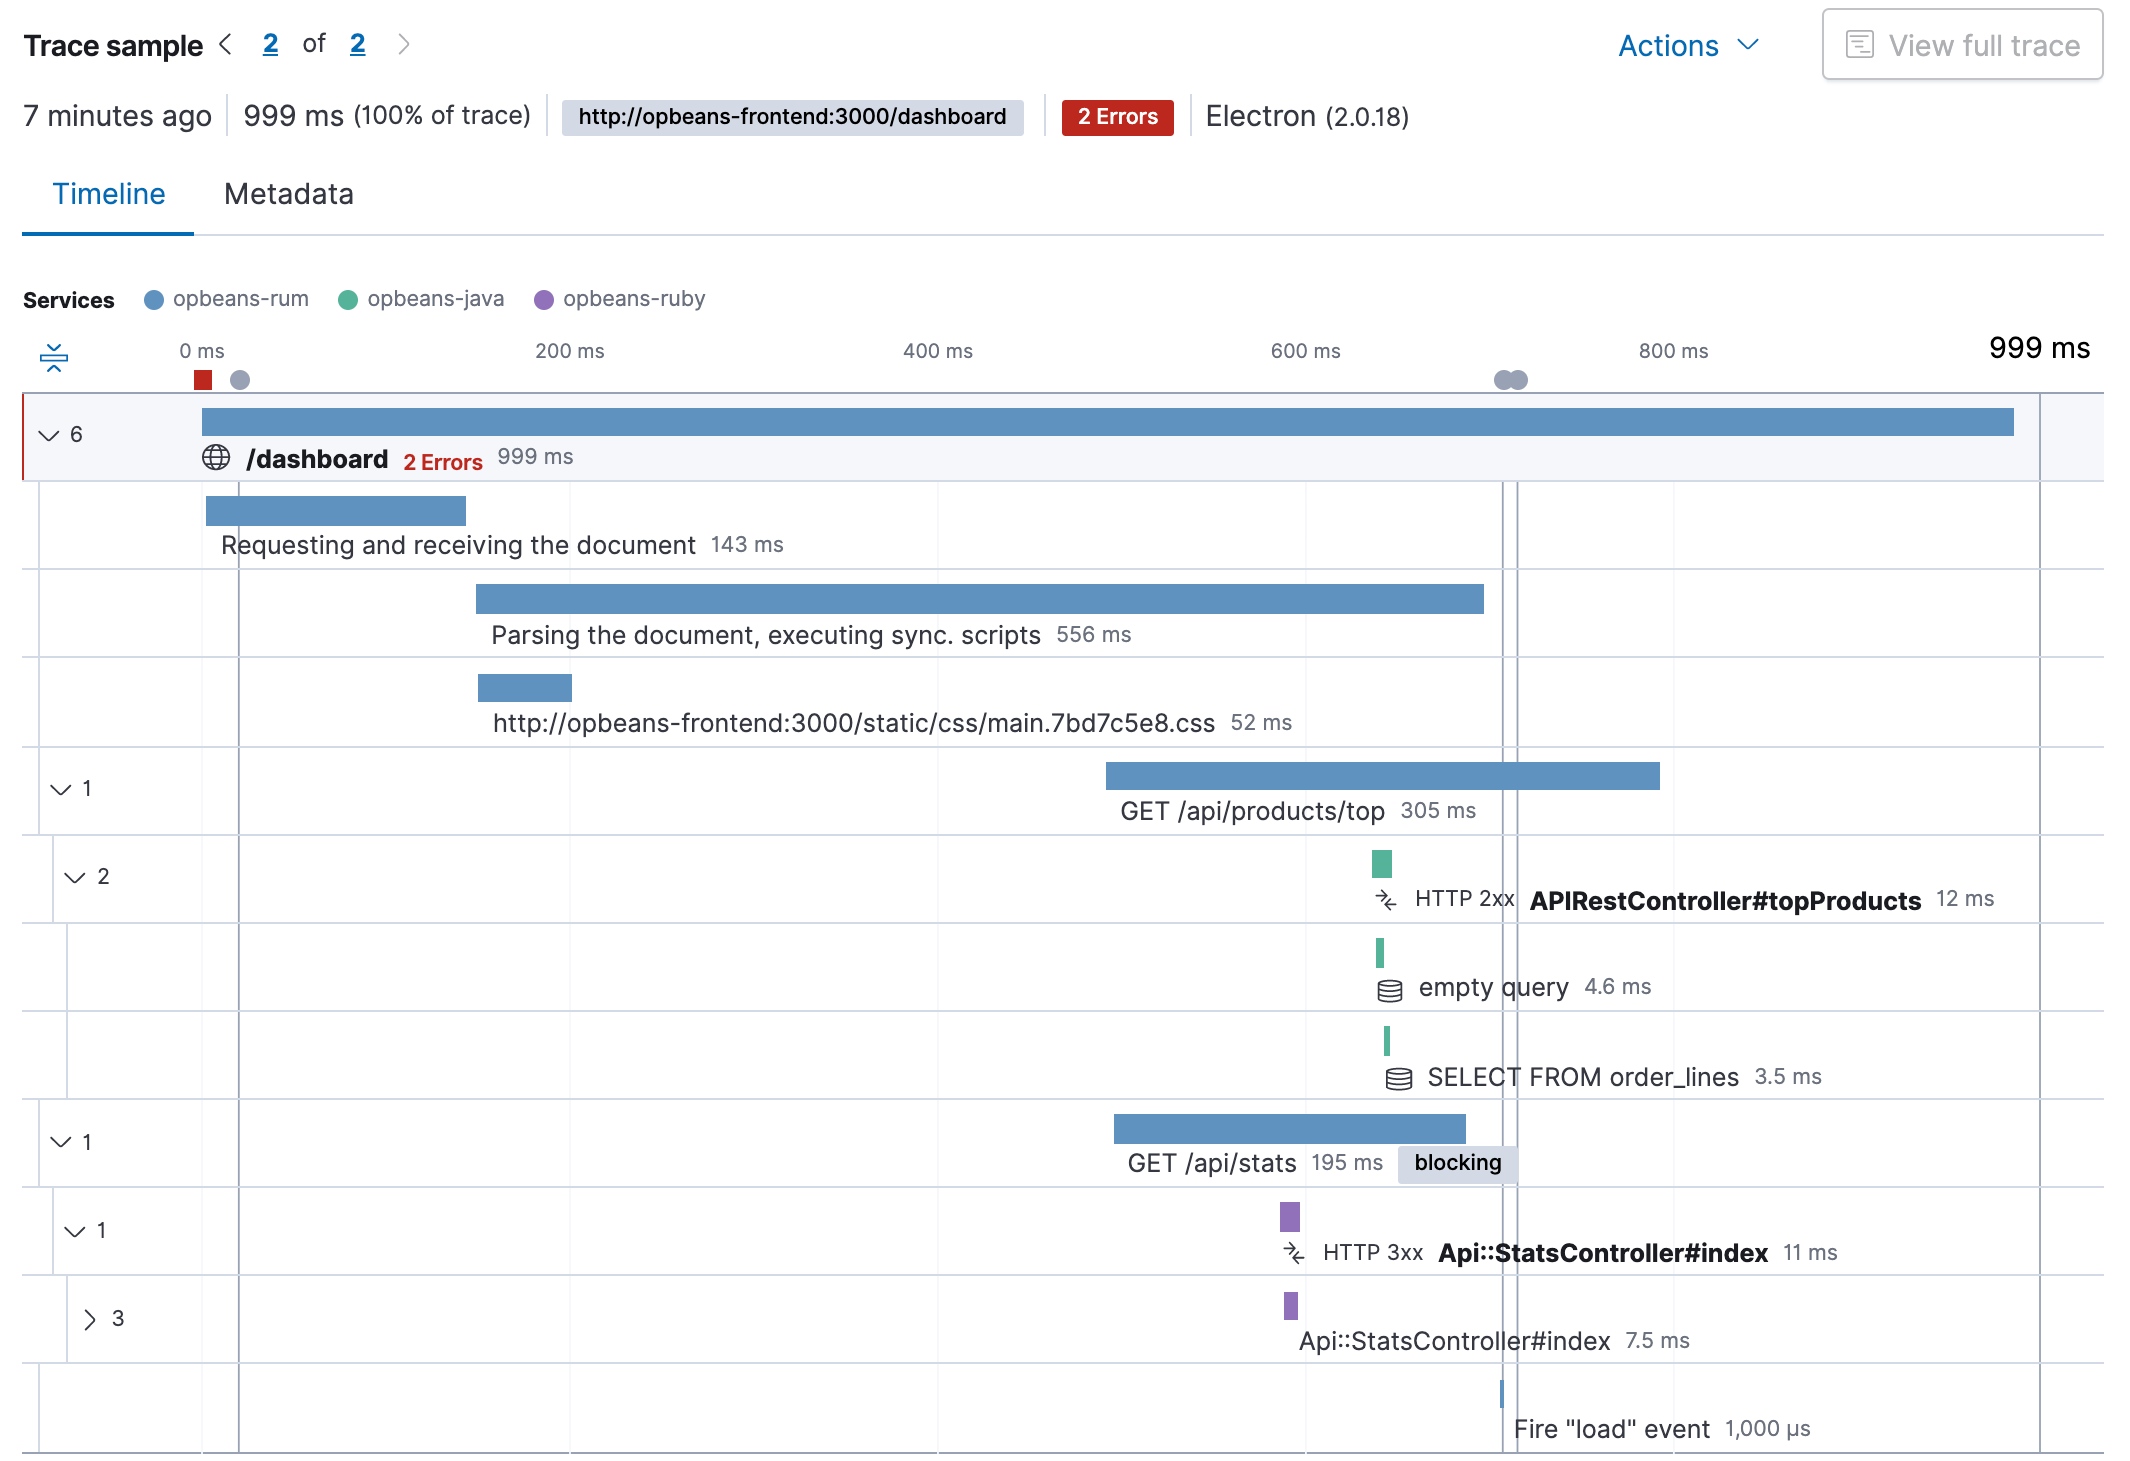
\includegraphics[height=0.7\textheight]{images/T7/tracing.png}
    \caption{Trace in Elastic APM. Source: \href{https://www.elastic.co/docs/solutions/observability/apm/traces}{Elastic APM documentation}.}
  \end{figure}

\end{frame}

\begin{frame}
  \frametitle{Observability: Logging}

  \begin{figure}
    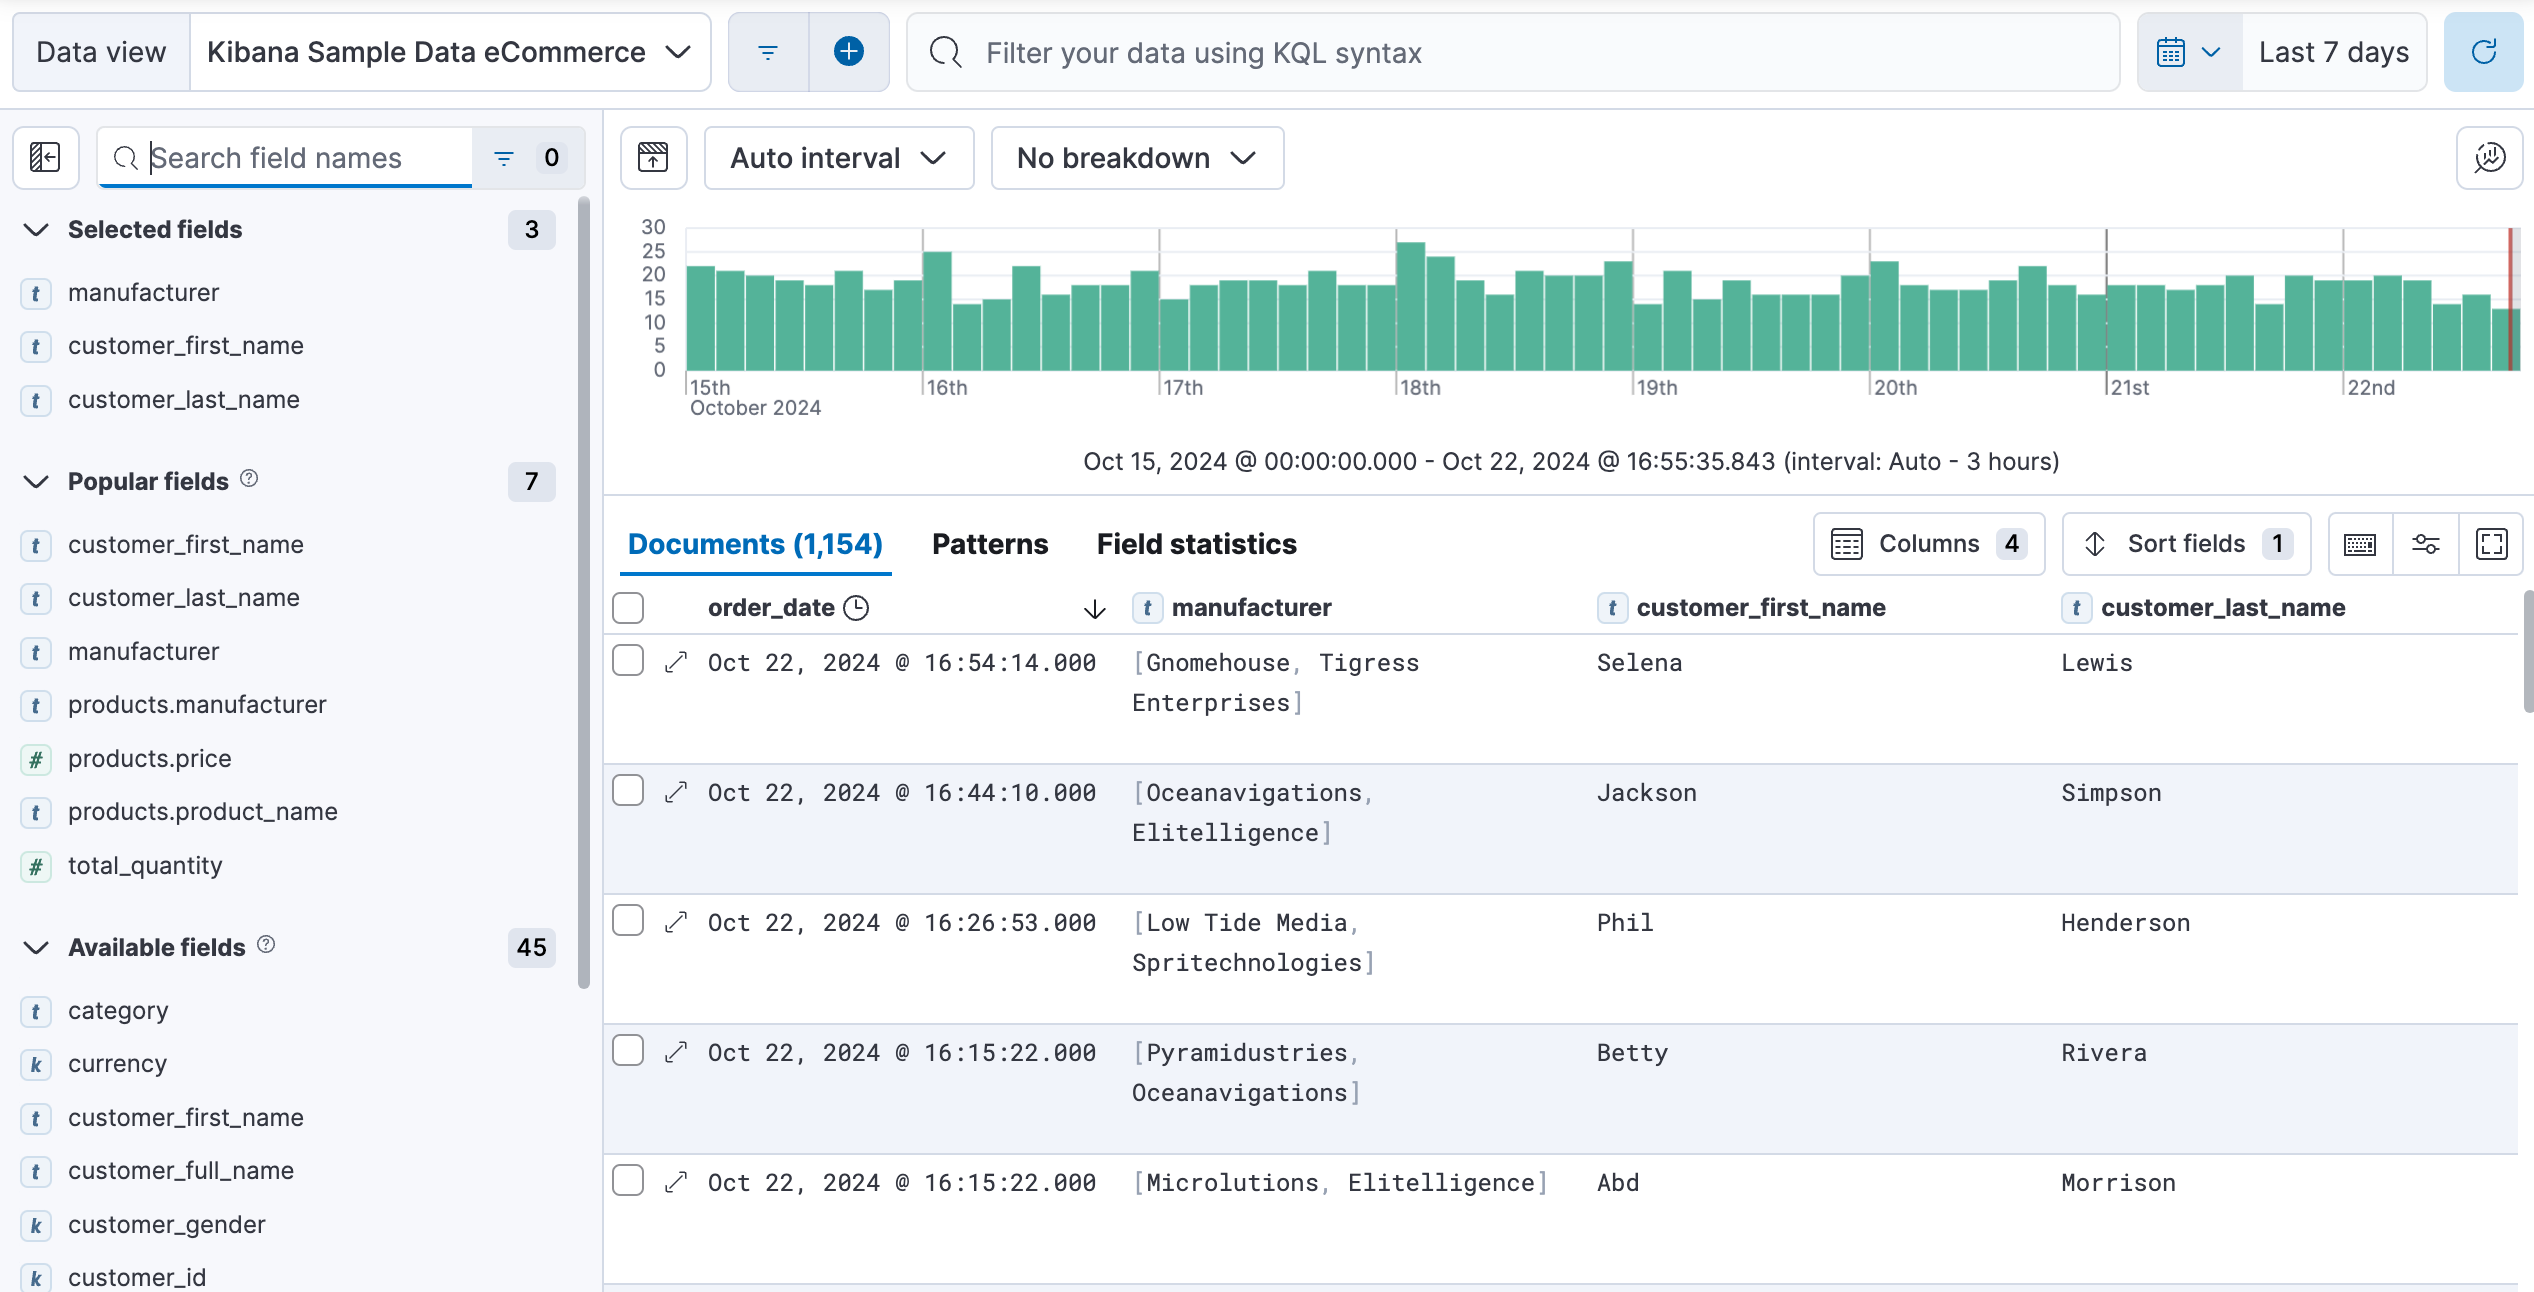
\includegraphics[height=0.67\textheight]{images/T7/logging.png}
    \caption{Logs in Kibana. Source: \href{https://www.elastic.co/docs/explore-analyze/discover/discover-get-started}{Kibana documentation}.}
  \end{figure}

\end{frame}

\begin{frame}
  \frametitle{Observability: Metrics}

  \begin{figure}
    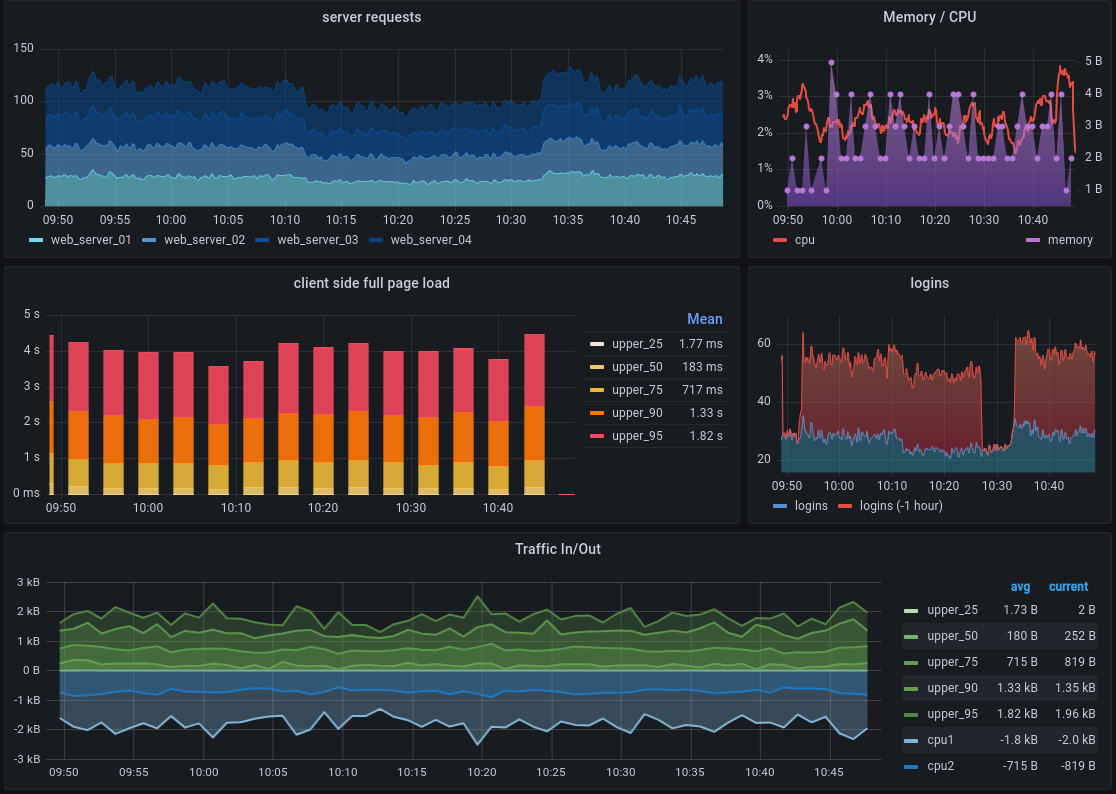
\includegraphics[height=0.7\textheight]{images/T7/metrics.png}
    \caption{Metrics in Grafana. Source: \href{https://grafana.com/docs/grafana-cloud/introduction/metrics-and-visualizations/}{Grafana Cloud documentation}.}
  \end{figure}

\end{frame}

\end{document}
